\section{O futuro do trabalho}
%%%%%%%%%%%%%%%%%%%%%%%%%%%%%%%%%%%%%%%%%%%%%%%%%%%%%%%%%%%%%%%%%
\qquad Agora com as novas tecnologias tem se aberto várias portas para novas formas de as pessoas poderem ser remuneradas por seus serviços ou bens. Exemplos muito notórios são casos como a UBER, AMAZON, YOUTUBE, LINKEDIN, etc, etc.
\emptyline
Esta a fugir para uma forma de trabalhadores independentes, subcontratados e de trabalho temporário, controlado por sistemas tecnológicos administrativos, empresas virtuais, que pode ser formas de exploração e concorrência desleal, quando mal usados, e proporcionam enriquecimento rápido aos que implementem estes sistemas e gerem.
\emptyline
Esta ideia já tinha surgido décadas atrás, como uma forma de reduzir custos e responsabilidade do cliente, como a agência de trabalho temporário \textbf{KELLY SERVICES} tinha publicado em 1971 acerca da oferta do tipo de trabalhadores que tinham ao dispor: \cite{book-11}
\emptyline
\hspace*{.5cm} - Nunca tiram feriados ou férias\\
\hspace*{.5cm} - Nunca pedem aumentos salariais\\
\hspace*{.5cm} - Nunca custa um cêntimo com folgas de trabalho\\
\hspace*{.5cm} - Nunca fica gripado, problemas de coluna ou dor de dentes\\
\hspace*{.5cm} - Nunca te chateia com situação de desemprego, impostos e segurança social\\
\hspace*{.5cm} - Nunca se cansam de satisfazer
\emptyline
Também poderia-se falar do caso da UBER na qual resultou em diversos processos em tribunal.
\emptyline
Estes acontecimentos servem de exemplo para que a sociedade tenha fortes Leis do trabalho, Direitos humanos e a obrigação de ter líderes conscientes.
\emptyline
Agora como foi abordado alguns pontos negativos que se podem encontrar no mundo de trabalho, já se sabe que o mundo foi feito para o ser humano, na qual todos nós somos ao mesmo tempo trabalhadores e clientes, e pretende-se que haja segurança e estabilidade para todos, cada vez mais se valoriza a liberdade, sendo que a esperança no mundo do trabalho seja para exterminar situações de exploração e corrupção.
\emptyline
Com a modernização existe uma especial preocupação com a classe trabalhadora com menos formação e a desigualdade na valorização laboral, sendo que quanto maior a procura com menor oferta tem maior o valor.
\emptyline
No caso de \textcolor{green}{Portugal} o futuro de trabalho esta muito bem estabelecido, esta tabelado, é uma economia por classes onde o governo trabalha de mãos dadas com as organizações, e a classe trabalhadora como é explicito é para trabalhar e manter o sistema a tona da água, seus vencimentos são controlados monitorizados de forma a garantir a competição internacional e sua sobrevivência, apenas os quadros superiores e de liderança tem direito a distribuição dos lucros, ou seja, os \textit{shareholders}.
\newpage
Abaixo uma tabela pré-definida de vencimentos para as universidades:\\
\begin{figure}[H]
	\centering
	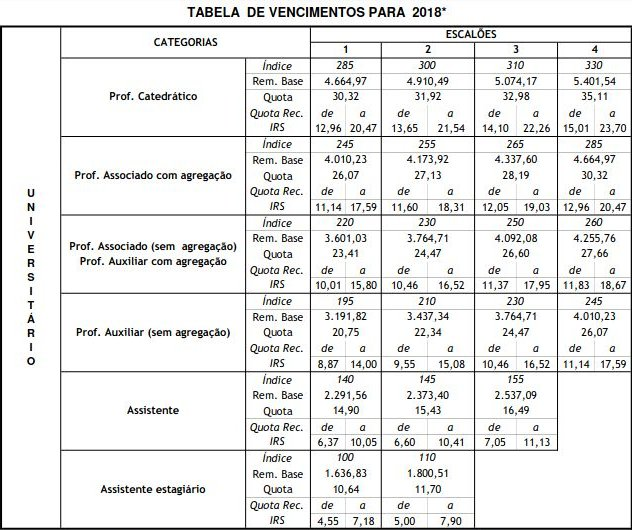
\includegraphics[scale=0.52]{./image/Salary/Universidade.jpg}
	\caption{Tabela de Vencimentos para 2018 \cite{article-2}}
\end{figure}
Estas publicações são expostas nos Diários da Republica e consequentemente nos Decretos de Lei, claro que quem cria este controle é quem tem os melhores vencimentos, todas as profissões são tabelados com um teto máximo de vencimento, dai que se diz que \textit{"Ninguém fica rico a trabalhar"}, toda a classe trabalhadora seu patronato é o Estado, ou seja, o Governo. As Organizações são Sócios do Governo e pagam uma taxa do uso dos seus cidadãos. Estas são deduções evidentes, temos exemplos como a \textit{TAP}, \textit{GALP}, \textit{NOVO BANCO}, as ajudas ás \textit{Pequenas e Médias Empresas}, dá a entender que o governo distribui a riqueza entre as organizações e em contrapartida estas gerem a população dando-lhes trabalho, o que é exposto neste relatório tem muita resistência na sociedade, dando a origem a perseguição e tortura pelo sistema instalado, racismo. \textcolor{green}{Portugal} vai receber ajuda da União Europeia na quantia de 15,5Mil Milhões de Euros a \textit{Fundo Perdido} e as famílias e a classe trabalhadora não vai ter direito as ajudas, mas ser explorados com essas verbas.
\newpage
No caso dos Engenheiros Eletrotécnicos:\\
\begin{figure}[H]
	\centering
	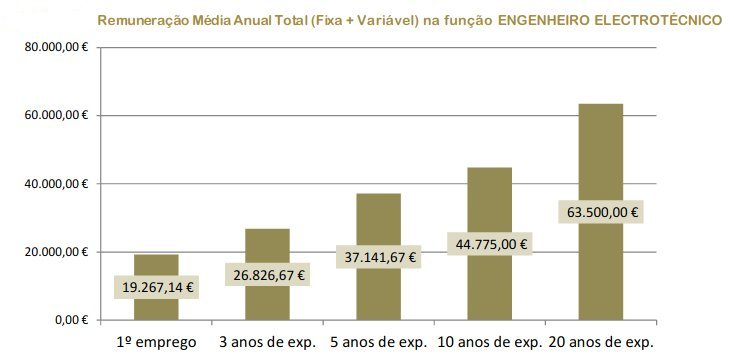
\includegraphics[scale=0.52]{./image/Salary/Eng_Elec.jpg}
	\caption{Tabela de Vencimentos para 2018 \cite{article-3}}
\end{figure}
Intervalo salarial máximo e mínimo da maioria dos trabalhadores da profissão Engenheiros Eletrotécnicos - a partir de \euro 5,24 até \euro 16,17 por hora - Ano 2020.\\
\textcolor{green}{[ link: \quad  https://meusalario.pt/emprego/portugal-emprego-e-salario/engenheiros-electricos ]}
\emptyline
Dai em Portugal o futuro do trabalho é incerto, e tudo depende do governo, isto é, da Cultura de Portugal.
\newpage
\section{A gestão de carreira e as competências necessárias num mundo em mudança}
%%%%%%%%%%%%%%%%%%%%%%%%%%%%%%%%%%%%%%%%%%%%%%%%%%%%%%%%%%%%%%%%%
A Industria tende a ser cada vez mais automatizada, e a mão de obra substituída por maquinas, as empresas estão a ser cada vez mais digital.
\emptyline
No futuros os empregos com melhores vencimentos vão ser nas áreas tecnológicas.\\
%\renewcommand{\labelitemi}{$\blacksquare$}
\begin{center}\textbf{\large Competências Consideradas no Estudo OCDE} % \cite{article_1}
\end{center}
\begin{minipage}[t]{.5\linewidth}
\qquad \textbf{Competências Cognitivas:}
\begin{itemize}
%\setlength\itemsep{-1em}
\item Numeração:\\
- Números\\
- Contar\\
- Aritmética
\item Literacia:\\
- Falar, Ler, Escrever, Línguas
\item Resolução de problemas:\\
- Raciocínio\\
- Lógica\\
- Silogismo\\
- Método Socrático\\
- Critica Interrogativa\\
- etc
\end{itemize}
\qquad \textbf{Competências Socioeconómicas:}
\begin{itemize}
\setlength\itemsep{-.5em}
\item Identidade
\item Formação Académica
\item Experiência Profissional
\end{itemize}
\qquad \textbf{Personalidade:}
\begin{itemize}
\setlength\itemsep{-.5em}
\item Facilidade de adaptação
\item Facilidade de aprendizagem
\item Imaginação
\item Estabilidade Emocional
\end{itemize}
\end{minipage}
\begin{minipage}[t]{.5\linewidth}
\qquad \textbf{Competências Operacionais:}
\begin{itemize}
%\setlength\itemsep{-0.8em}
\item Gestão e Comunicação:\\
- Planear, Organizar, Controlar, etc\\
- Comunicação formal e informal
\item Contabilidade e Vendas:\\
- Marketing Mix\\
- Analise de Parêto\\
- etc
\item Organização Pessoal:\\
- Diagrama de Gantt\\
- Analise de Parêto\\
- etc
\item Numeração Avançada:\\
- Aritmética, Álgebra, Geometria\\
- Trigonometria, Cálculos\\
- Sistemas Dinâmicos\\
- Estatística\\
- etc
\item Tecnologias de informação e comunicação:\\
- Computadores, Telemóvel\\
- Internet, e-mail\\
- Programação\\
- Telecomunicações\\
- etc
\end{itemize}
\end{minipage}
\minipagespace{.3cm}
Acima esta um conjunto de competências que pelos estudos efetuados demonstrou que trabalhadores da industria com maior intensidade digital em média exibem maiores níveis de competência cognitiva e também operacionais do que os trabalhadores nos sectores económicos de menor intensidade digital. Isto claro depende do tipo de trabalhador empregue no sector digital versus o de menor intensidade digital, em que o segundo geralmente são trabalhadores sem qualificações. \cite{article-1}\\
Também é demonstrado que todas as competências tem maior recompensa nas industrias digitalmente intensificadas, particularmente numeração avançada, organização pessoal, tecnologias de informação e comunicação e numeração. \cite{article-1}\\
A recompensa de vencimento pela competência de tecnologias de informação e comunicação é o dobro em relação a competência de numeração, e aonde competências de gestão e comunicação tem recompensa igual as de numeração. \cite{article-1}\\
As competências operacionais ainda estão ao mesmo nível das cognitivas demonstrando forte evidencia da importância de trabalhos orientados a tarefa no mercado de trabalho. \cite{article-1}\\
Compreender quais a competências, tanto como as cognitivas e operacionais, quais são melhor recompensados financeiramente também é importante para responder aos assuntos de  desigualdades e criar empregos e bem estar. A falta da oferta de competências ou conjunto de competências pode facilmente criar desigualdade salarial e desemprego dos trabalhadores sem esses tipos de competências, dai a importância de criar programas de formação para preparar os trabalhadores nessas competências de alta procura dado a aceleração da transformação digital transversal nas ocupações e industria. E quanto mais cedo começa esse treinamento menor os custos de formação das competências necessárias. \cite{article-1}
\emptyline
A industria mais tecnologicamente digital paga melhor seus trabalhadores, a formação e treino é necessário para adquirir as competências desejadas para poder prosperar no mercado de trabalho.
%%%%%%%%%%%%%%%%%%%%%%%%%%%%%%%%%%%%%%%%%%%%%%%%%%%%%%%%%%%%%%%%%
%%%%Plano de Careira%%%%
\section{Plano de desenvolvimento pessoal de competências}
\qquad O meu plano de desenvolvimento pessoal, passa por obter mais formação e aprender com pessoas com mais experiência em diversas áreas, que é exatamente o que estou a fazer frequentando o curso de Engenharia Eletrotécnica e de Computadores no \textcolor{gray}{I.S.E.P}.\\
Esta disciplina em particular é uma forma de poder enriquecer minhas competências e metodologias de Gestão, e perceber as restantes matérias abordadas que compõem o \textcolor{blue}{Comportamento Organizacional}.\\
\begin{minipage}{8.5cm}
	\textbf{Metodologias da gestão}: \cite{book-9}
	\emptyline
	\begin{minipage}{3.1cm}
		Instrumental
		\begin{enumerate}
			\setlength\itemsep{-0.3em}
			\item Planear
			\item Organizar
			\item Controlar\\
		\end{enumerate}
	\end{minipage}
	\begin{minipage}{5cm}
		Comportamental
		\begin{enumerate}
			\setlength\itemsep{-0.3em}
			\item Liderança
			\item Comunicação
			\item Motivação
			\item Tomada de decisão
		\end{enumerate}
	\end{minipage}
\end{minipage}
\begin{minipage}{10cm}
\begin{figure}[H]
	\flushleft
	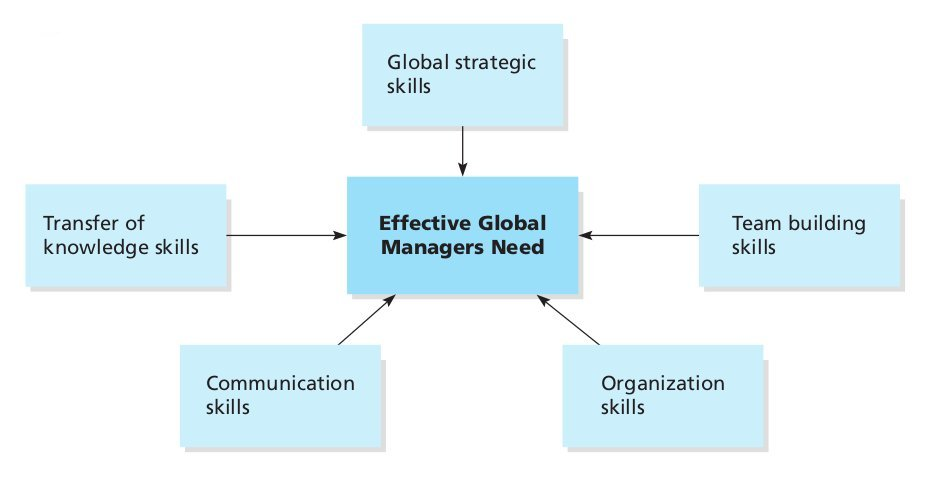
\includegraphics[scale=0.3]{./image/Skills/Managerial_Skills_for_the_Global_Marketplace.jpg}
	\caption{Competências de Gestão. \cite{book-6}}
\end{figure}
\end{minipage}
\emptyline
No entanto por enquanto minha missão é concluir a formação, e ao mesmo tempo melhorar um conjunto de ferramentas e métodos de trabalho para que seja estável e eficaz de forma a poder resolver os problemas que possa ter que enfrentar com facilidade, e eventualmente realizar alguns projetos pessoais.
\newpage
\subsection{Análise S.W.O.T Pessoal}
\qquad Neste contexto de plano de desenvolvimento a análise \textcolor{blue}{SWOT} também pode ser uma ferramenta útil de forma a nos indicar qual os comportamentos que poderá ser melhorado ou alterado.
\emptyline
\fbox{
\begin{minipage}[t]{\linewidth}
\begin{itemize}
	\setlength\itemsep{-0.85em}
	\item \textcolor{purple}{I}nterno
	\begin{itemize}
		\setlength\itemsep{-0.3em}
		\item \textcolor{orange}{S}trength (forças) \\
		- Numeração, Literacia Bilingue, Resolução de Problemas \\
		- Formação Académica, Experiência Profissional \\
		- Facilidade de Adaptação e aprendizagem, Imaginação \\
		- Gestão e Comunicação, Organização Pessoal \\
		- Numeração Avançada, Tecnologias de informação e comunicação. \\
		- Estabilidade Emocional \\
		- Empatia, Método Cientifico
		\item \textcolor{orange}{W}eakness (fraquezas) \\
		- Contabilidade e Vendas \\
		- Direto, Crítico, Detesto desigualdade e injustiças \\
		- Frontal com contradições \\
		- "Dente por dente e olho por olho" \\
		- Anti-Dogma
	\end{itemize}
	\item \textcolor{purple}{E}xterno
	\begin{itemize}
		\setlength\itemsep{-0.3em}
		\item \textcolor{orange}{O}pportunity (oportunidades) \\
		- Nenhum
		\item \textcolor{orange}{T}hreats (ameaças) \\
		- Cultura Portuguesa \\
		- Sistema Político-Social \\
		- Racismo
	\end{itemize}
\end{itemize}
\end{minipage}
}
\emptyline
Algumas explicações de personalidade descrevo no caso de quando se diz "dente por dente e olho por olho", muitas das vezes tem interpretação errada, pois concluem que existiria apenas cegos após alguns tempos, mas sendo uma metáfora, sabe-se que ninguém vai andar a cegar uns aos outros sem motivo e são circunstancias de saber individual, mas deve ser percebido no aspeto em que uma pessoa que é honesta merece honestidade, e uma humilde humildade, e pelo verso um mentiroso aldrabado, e assassino deve ser morto, este procedimento leva com que o bem vence sempre, isto é lógico e citações milenares de certa forma condiz neste caso. Que levanta também a questão da veracidade da perceção, na qual muito cuidado é exigido. \\
Dai que certas pessoas quando estão a ser irónicas, acabam dececionados com as reações esperadas, podendo entrar em ciclos viciosos que só vão agravando.
\emptyline
Quanto ao método cientifico nos diz que se um acontecimento se repete nas mesmas circunstâncias e nunca se altera é considerado facto ou lei ou teoria, é uma arte de reconhecer padrões. Também nós ensina que os conhecimentos estão sempre abertos ao escrutínio e se houver prova que refuta a teoria esta deixa de o ser, ou seja, é tentar representar a realidade observada por modelos racionais e matemáticos, as ferramentas que estão ao nosso dispor, já que não existe melhor.
\emptyline
Acho que esta análise seria mais prudente se fosse feito por uma perspetiva de terceiros, pois nos faria refletir nossas próprias preposições podendo ser reforçado ou até alterado.
\subsection{Curriculum Vitae}
\qquad Curriculum vitae significa "percurso de vida" \; em latim, ao primeiro era pouco conhecido e pouco utilizado, ou reservado apenas a uma fração da população ativa, principalmente aos jovens diplomados ou aos quadros que mudavam de "situação". No entanto os tempos mudaram devido a instabilidade e mudanças que levou a grande procura de novos empregos com muitos candidatos e o principal documento que terá os elementos fundamentais, que conduzem à apreciação e seleção é, sem dúvida, o CV.\cite{book-12}
O CV é um meio que permite a comunicação, para transmitir tua experiência profissional, tua personalidade na qual deve mencionar tuas motivações e objetivos algo que poderá separar dos restantes candidatos. \\
O Papel do CV serve para sermos selecionados para uma eventual entrevistas de trabalho, e consequentemente obter um acordo ou contrato de trabalho. Este documento é sempre um anexo nas candidaturas por qualquer via de comunicação, seja por e-mail ou contacto direto. \\
O CV em princípio deve conter tua identificação, morada, formação académica e literária, personalidade, experiência profissional e outros assuntos relacionados, ou seja, acaba por ser uma forma de divulgar as tuas competências de forma ordenada e organizada, para ser apelativo deve ser percetível e suscito, na qual só uma observação rápido pode ter uma ideia geral do candidato.
\emptyline
\textit{Anexado CV}.

